\chapter{Triangle Center}% by Saad Bin Quddus

\begin{linkb}
   \begin{itemize}
       \item \href{https://www.youtube.com/watch?v=gWAeVwjzndQ}{Triangle Center (Saad)}
        \item \href{https://drive.google.com/file/d/1JISJtfI-zb_jadi_gM5iWcz1ao4Dw4J8/view}{Triangle Center Pset}
   \end{itemize}
\end{linkb}



Today's topic is about basic triangle centers like circumcenter, centroid, incenter, excenter, orhtocenter, etc\ldots (This is mostly Angle Chasing in a TRIANGLE)



\section{Circumcenter}
I think, you are familiar with the circumcenter. It is the center of the circle which goes through the points $A,B,C$ of $\triangle ABC$. It is determined by drawing the perpendicular bisectors of the line segments.

\begin{figure}[ht] 
\centering
	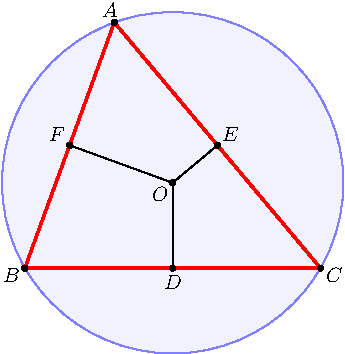
\includegraphics{circum.pdf}
\caption{Circumcenter of \(\triangle ABC\)}
\end{figure}
The proof of concurrency is very easy. Just remember that any point on the perpendicular bisector is equidistant from two of the corresponding vertex. 
%He showed the proof of concurrency of the perpendicular bisector of the sides of a triangle. I am not going to include the proof as you can find it in anywhere. 

\section{Centroid}

Centroid is the intersection of the medians of a triangle. It is defined by \(G\). It is also called Center of Mass or Center of Gravity.
\begin{figure}[h]
	\centering
	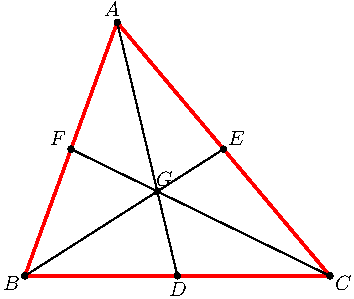
\includegraphics{centroid.pdf}
\caption{Centroid of \(\triangle ABC\)}
\end{figure}


Here we are going to see a combinatorial proof!

Let, three centroid don't concur, then they intersect in three pints let \(G_1,G_2,G_3\). Let 
the midpoints of the sides are \(L,M,N\). Then draw the medians of the triangle \(LMN\) then, 
their medians intersect at \(G_1,G_2,G_3\) as \(MN\parallel BC\). So we are going to infinite 
descent, and consider the median triangle of \(LMN\). Consequently, the areas of the median 
triangles are going to \(0\). But the area of triangle \(G_1G_2G_3\) remains same. which means 
triangle \(G_1G_2G_3\) is bigger that the original triangle which is a contradiction. So 
centroid exists. 


\section{Orthocenter}

Let \(D,E,F\) be the foot of the perpendicular from \(A,B,C\) to the opposite side of the 
triangle. Then \(BFEC\) is a cyclic quadrilateral(You can see this by \(\angle FEA = B\) or by 
\(\angle BFC = \angle BEC =90\dg\)). Also there are another two cyclic quadrilaterals. Find them.


\begin{figure}[ht]
%\centering
\begin{center}
	\begin{minipage}[t]{6.5cm}
		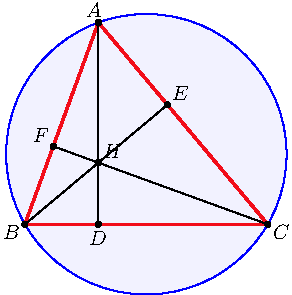
\includegraphics{ortho.pdf}
	\\ \centering \sffamily Orthocenter of \(\triangle ABC\)
	\end{minipage}
		\quad
	\begin{minipage}[t]{6.5cm}
		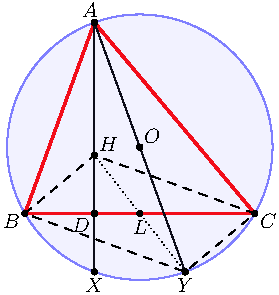
\includegraphics{ortho-reflect.pdf}
	\\ \centering \sffamily Reflection of Orthocenter lies on Circumcirlce
	\end{minipage}
\end{center}	
\caption{Ortocenter and its Reflections}
\end{figure}

There are six cyclic quadrilaterals and the orthocenter is the incenter of the orthic trinagle.


\begin{figure}[ht] 
\centering
		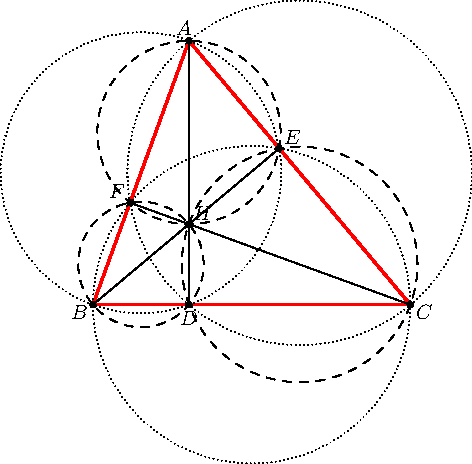
\includegraphics{ortho-6cyclic.pdf}
\caption{Orthocenter and 6 cyclic quadrilaterals}
\end{figure}

Then Mentor taught us the reflection of the orthocenter across the sides and about the midpoint of the sides lie on the circumcircle of the triangle \(ABC\). 
Let the reflection of \(H\) across the side \(BC\) is \(X\) then we are going to show that \(X\) lies on \((ABC)\). 

Note that \(\triangle BDH \cong \triangle BDX\) by some angle chasing.

So, \(\angle BXH = \angle BHD = \angle ACB\) and therefore \(ABXC\) is a cyclic quadrilateral.

Let the reflection of H acroos the midpoint of \(BC\) is \(Y\).
Then, \[\angle BAH = \angle CAO=90\dg - B.\]
and \(AY\) is a diameter.

\(BH=CY\) hence, \(BH\parallel CY\) thererfore, \(BHCY\) is a parallelogram, and \(H,L,Y\) are collinear. hence \(Y\) lies on \((ABC)\).




\section{Nine Point Circle}
Our current topic is the famous Nine-Point Circle whih goes through exactly nine points.

These pints are three midpoints, three feet of the perpendicular and the three midpoints of \(AH,BH,CH\).

Now we are going to show the first six points are concyclic.
%npc
\begin{figure}[ht] 
\centering
		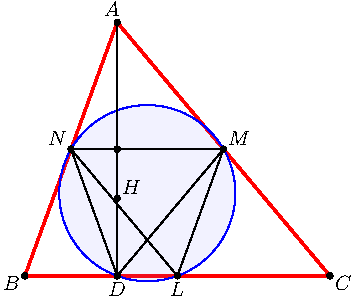
\includegraphics{npc-proof.pdf}
\caption{\(D,L,M,N\) lie on a circle}
\end{figure}
\(D\) is the reflection of \(A\) across \(MN\)
so \(\angle MDN = A\) we also know that \(\angle MLN = A\) so \(L,M,N,D\) are concyclic . Similarly we can show that \(L,M,N,E\) and \(L,M,N,F\) are concyclic, so all six points are concyclic.
Other proof \(\angle BDN = \angle NML\) so \(L,M,N,D\) are concyclic points.


Now we are gonna prove that \(K\) the midpoint of \(AH\) lies on \((DEFLMN)\). 
\(\angle NLB = C \) so we have to show that \(\angle NKH = C\). but \[ \angle NKH= \angle BHD = C\] so we are done.

Also \(N_9\) the center of the Nine-Point Circle is the midpoint of \(OH\) where \(O\) and \(H\) are circumcenter and Orthocenter respectively.

%npc
\begin{figure}[ht] 
\centering
	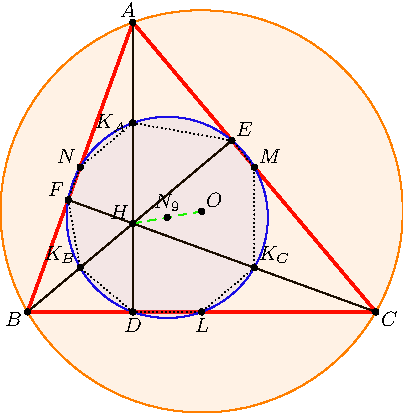
\includegraphics{npc-full.pdf}
\caption{Nine Point Circle of \(\triangle ABC\)}
\end{figure}


\section{Practice Problems}

\begin{problem}
Let $H$ be the orthocenter of triangle $ABC$ and $D,E,F$ be the feet of the perpendicular on the sides $BC,CA,AB$. Prove that $H$ is the incenter of triangle $DEF$.
	\begin{hint}
		\addhint{ }
		\addhint{ }
		%\addhint{Solution at \url{}}
	\end{hint}
\end{problem}

\begin{problem}
Prove that the reflection of the \textit{Euler Line} on the sides of $\triangle ABC$ concur at the circumcircle.
	\begin{hint}
		\addhint{ }
		\addhint{ }
		%\addhint{Solution at \url{}}
	\end{hint}
\end{problem}

\begin{problem}[2020 China North Mathematical Olympiad (Basic) P4]
In $\triangle ABC$, $\angle BAC = 60^{\circ}$, point $D$ lies on side $BC$, $O_1$ and $O_2$ are the centers of the circumcircles of $\triangle ABD$ and $\triangle ACD$, respectively. Lines $BO_1$ and $CO_2$ intersect at point $P$. If $I$ is the incenter of $\triangle ABC$ and $H$ is the orthocenter of $\triangle PBC$, then prove that the four points $B,C,I,H$ are on the same circle.
	\begin{hint}
		\addhint{ }
		\addhint{ }
		\addhint{Solution at \url{https://artofproblemsolving.com/community/c6h2220889p16882243}}
	\end{hint}
\end{problem}

\begin{problem}[Swiss MO 2007/4]
Let $ABC$ be an acute-angled triangle with $AB> AC$ and orthocenter $H$. Let $D$ the projection of $A$ on $BC$. Let $E$ be the reflection of $C$ wrt $D$. The lines $AE$ and $BH$ intersect at point $S$. Let $N$ be the center of $AE$ and let $M$ be the midpoint of $BH$. Prove that $MN$ is perpendicular to $DS$.
	\begin{hint}
		\addhint{ }
		\addhint{ }
		\addhint{Solution at \url{https://artofproblemsolving.com/community/c6h2197471p16518225}}
	\end{hint}
\end{problem}

\begin{problem}[British MO 1981 P1]
$H$ is the orthocentre of triangle $ABC$. The midpoints of $BC, CA, AB$ are $A', B', C'$ respectively. A circle with centre $H$ cuts the sides of triangle $A'B'C'$ (produced if necessary) in six points, $D_1, D_2$ on $B’C'$,$E_1, E_2$ on $C'A'$ and $F_1, F_2$ on $A'B'$. Prove that, $AD_1=AD_2=BE_1=BE_2=CF_=CF_2$.
	\begin{hint}
		\addhint{ }
		\addhint{ }
		\addhint{Solution at \url{https://artofproblemsolving.com/community/c6t70430f6h2531807_ad_1ad_2be_1be_2cf_cf_2_wanted_circle_center_h_through_6_points}}
	\end{hint}
\end{problem}

\begin{problem}[47th Austrian MO P2]
We are given an acute triangle $ABC$ with $AB > AC$ and orthocenter $H$. The point $E$ lies symmetric to $C$ with respect to the altitude $AH$. Let $F$ be the intersection of the lines $EH$ and $AC$. Prove that the circumcenter of the triangle $AEF$ lies on the line $AB$.
	\begin{hint}
		\addhint{ }
		\addhint{ }
		\addhint{Solution at \url{https://artofproblemsolving.com/community/c6h1681663p10722184}}
	\end{hint}
\end{problem}

\begin{problem}
Let $ABC$ be an acute triangle with orthocenter $H$ and circumcenter $O$. Let $K$ be the midpoint of the segment $AH$. Let $P$ be a point on $AC$ such that, $OP \parallel BC$. Show that $\angle BKP= 90^{\circ}$ 
	\begin{hint}
		\addhint{ }
		\addhint{ }
		\addhint{Solution at \url{https://artofproblemsolving.com/community/q1h2353259p19090174}}
	\end{hint}
\end{problem}

\begin{problem}[2017 Saudi Arabia JBMO TST P7]
Let $ABC$ be a triangle inscribed in the circle $(O)$, with orthocenter $H$. Let d be an arbitrary line which passes through $H$ and intersects $(O)$ at $P$ and $Q$. Draw diameter $AA'$ of circle $(O)$. Lines $A'P$ and $A'Q$ meet $BC$ at $K$ and $L$, respectively. Prove that $O, K, L$ and $A'$ are concyclic.
	\begin{hint}
		\addhint{ }
		\addhint{ }
		\addhint{Solution at \url{https://artofproblemsolving.com/community/c6h2124972p15486860}}
	\end{hint}
\end{problem}

\begin{problem}[2019 Romania JBMO TST Day 2 P3]
Let $d$ be the tangent at $B$ to the circumcircle of the acute scalene triangle $ABC$. Let $K$ be the orthogonal projection of the orthocenter, $H$, of triangle $ABC$ to the line $d$ and $L$ the midpoint of the side $AC$. Prove that the triangle $BKL$ is isosceles.
	\begin{hint}
		\addhint{ }
		\addhint{ }
		\addhint{Solution at \url{https://artofproblemsolving.com/community/c6h2135307p15639880}}
	\end{hint}
\end{problem}

\begin{problem}[Ukraine TST 2014 p4]
The $A$-excircle of the triangle $ABC$ touches the side $BC$ at point $K$. The circumcircles of triangles $AKB$ and $AKC$ intersect for the second time with the bisector of angle $A$ at points $X$ and $Y$ respectively. Let $M$ be the midpoint of $BC$. Prove that the circumcenter of triangle $XYM$ lies on $BC$.
	\begin{hint}
		\addhint{ }
		\addhint{ }
		\addhint{Solution at \url{https://artofproblemsolving.com/community/c6h2082814p14992490}}
	\end{hint}
\end{problem}

\begin{problem}[2020 Nicaragua Iberoamerican MO TST]
Let $H$ and $O$ be the orthocenter and circumcenter of an scalene and acute-angled triangle $ABC$ with circumcircle $\Gamma$. Points $K$ and $M$ are the midpoints of $AH$ and $BC$, respectively. Let $L$ be a point on the circumcircle of $OAK$ so that $\angle ALM=90^{\circ}$.\\
    
If line $AO$ meets $\Gamma$ again at $D$, and line $AL$ meets $\Gamma$ again at $J$, show that $MD$ and $DJ$ are perpendicular to each other.
	\begin{hint}
		\addhint{ }
		\addhint{ }
		\addhint{Solution at \url{https://artofproblemsolving.com/community/c6h1993208p13898771}}
	\end{hint}
\end{problem}

\begin{problem}[2020 Estonia TST P4]
Let $O$ be the circumcenter and $H$ the orthocenter of an acute-triangle $ABC$. The perpendicular bisector of $AO$ intersects the line $BC$ at point $S$. Let $L$ be the midpoint of $OH$. Prove that $\angle OAH = \angle  LSA$.
	\begin{hint}
		\addhint{ }
		\addhint{ }
		\addhint{Solution at \url{https://artofproblemsolving.com/community/q1h2292197p18049462}}
	\end{hint}
\end{problem}

\begin{problem}[2016 Thailand TST Day 1 P1]
Let $\vartriangle ABC$ be an acute-angled triangle whose altitudes $AA_1$ and$ BB_1$ intersect at $H$. Let $\omega_1$ be the circle centered at $H$ passing through $B_1$ and let $\omega_2$ be the circle centered at $B$ passing through $B_1$. Let $CN$ and $CK$ be the tangent lines from $C$ to circles $\omega_1$ and $\omega_2$ respectively ($N$ and $K$ are distinct from $B_1$). Prove that $A_1, N$ and $K$ are collinear.
	\begin{hint}
		\addhint{ }
		\addhint{ }
		\addhint{Solution at \url{https://artofproblemsolving.com/community/c6h2315798p18441752}}
	\end{hint}
\end{problem}

\begin{problem}[USA TST 2011 P1]
In an acute scalene triangle $ABC$, points $D,E,F$ lie on sides $BC, CA, AB$, respectively, such that $AD \perp BC, BE \perp CA, CF \perp AB$. Altitudes $AD, BE, CF$ meet at orthocenter $H$. Points $P$ and $Q$ lie on segment $EF$ such that $AP \perp EF$ and $HQ \perp EF$. Lines $DP$ and $QH$ intersect at point $R$. Compute $HQ/HR$.
	\begin{hint}
		\addhint{ }
		\addhint{ }
		\addhint{Solution at \url{https://artofproblemsolving.com/community/c6h420422p2374795}}
	\end{hint}
\end{problem}

\begin{problem}[Canadian Buffet Contest 2021 G4]
In $\triangle ABC$, let $D$, $E$, $F$ be the feet of altitudes from $A$, $B$, $C$ respectively. Let $K$ be the orthocenter of $\triangle DEF$. Let $U$,$V$,$W$ be the projections of points $F$, $D$, $E$, on $BC$, $CA$, $AB$ respectively. Assume that the circumcircles of $\triangle ABC$ and $\triangle UVW$ intersect at two points $M$ and $N$, prove that $KM=KN$.
	\begin{hint}
		\addhint{ }
		\addhint{ }
		\addhint{Solution at \url{https://artofproblemsolving.com/community/c6t70430f6h2538253_on_the_properties_of_orthocenter_of_def}}
	\end{hint}
\end{problem}

\begin{problem}[Iran MO 3rd round 2018 G4]
For acute triangle $\triangle ABC$ with orthocenter $H$, and $E,F$ the feet of altitudes for $B,C$, we have $P$ on $EF$ such as that $HO \perp HP$. $Q$ is on segment $AH$ so $HM \perp PQ$. prove $QA=3QH.$
	\begin{hint}
		\addhint{ }
		\addhint{ }
		\addhint{Solution at \url{https://artofproblemsolving.com/community/c6t70430f6h1701020_iran_geometry_third_round_2018}}		
	\end{hint}
\end{problem}
%\section{}

%\includepdf[pages=-]{triangle-center-pset.pdf}

%\begin{soln}[to Problem 1.1]
%This is trivial. Just angle Chase.
%\end{soln}



